%!TEX root = ../../main.tex

%% Trabalhar aqui
Para a AlexNet, assim como para a CNN anterior, foi realizada uma busca em \emph{grid} com os hiperparâmetros selecionados anteriormente, com vistas a obter os melhores modelos para cada abordagem de separação de dados, gerando assim, mais $36$ modelos a serem avaliados quanto às suas métricas de desempenho.

Considerando a métrica de \emph{F-score}, foram selecionados os melhores modelos  desta arquitetura e estes encontram-se listados na Tabela \ref{tab:alexnet}. Na Figura \ref{fig:treinamento-alexnet} pode-se observar os gráficos com os comportamentos dos valores de \emph{loss} e acurácia encontrados nos conjuntos de treinamento e validação durante o estágio de treino destes modelos. Apenas para referência posterior, considerou-se uma rotulação das melhores redes identificadas.

\begin{table}[h!]
\centering
\caption{Detalhamento dos melhores modelos obtidos com a arquitetura AlexNet, organizados de forma decrescente considerando o valor de Acurácia.}
\label{tab:alexnet}
\begin{tabular}{cccccc}
\toprule
\textbf{Identificação} & \textbf{Otimizador} & \textbf{\emph{Patience}}  & \textbf{Função de Ativação} & \textbf{Acurácia} & \textbf{F-Score} \\
\midrule
AlexNet A & Adam & 15 & ELU & $0.9654$ & $0.9393$ \\
AlexNet B & SGD & 10 & \emph{Leaky} ReLU & $0.9601$ & $0.9311$ \\
AlexNet C & SGD & 5 & SELU & $0.9561$ & $0.9244$ \\
\bottomrule
\end{tabular}
\end{table}

\begin{figure}[H]
 \centering
 \caption{Histórico de \emph{loss} e acurácia durante o treinamento dos melhores modelos obtidos com a arquitetura AlexNet.}
 \label{fig:treinamento-alexnet}
 \subfloat[\emph{Loss} durante treinamento da rede AlexNet A.\label{subfig:alexnet-a-loss}]{%
 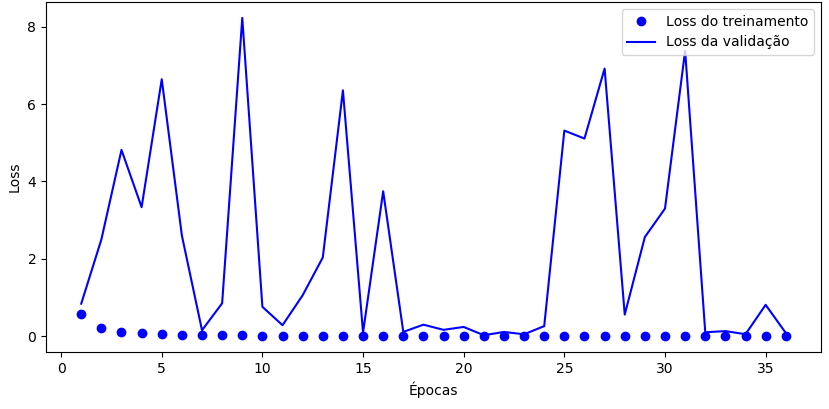
\includegraphics[width=0.45\textwidth]{imgs/alexnet-a-loss}
 }
 \subfloat[Acurácia durante treinamento da rede AlexNet A.\label{subfig:alexnet-a-acc}]{%
 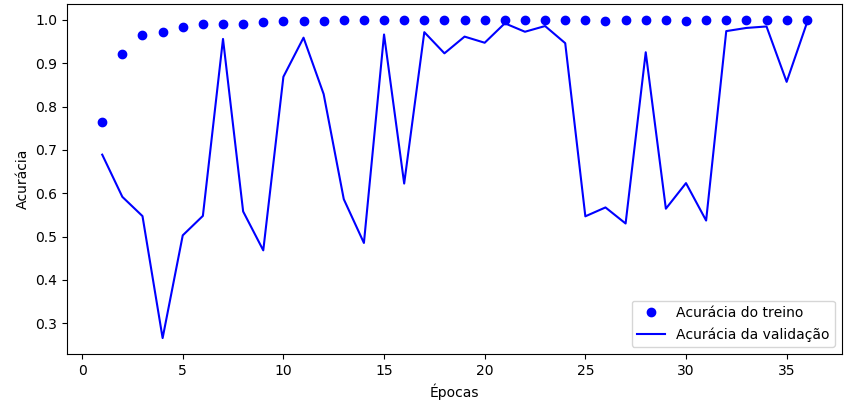
\includegraphics[width=0.45\textwidth]{imgs/alexnet-a-acc}
 }
 \hfill
 \subfloat[\emph{Loss} durante treinamento da rede AlexNet B.\label{subfig:alexnet-b-loss}]{%
 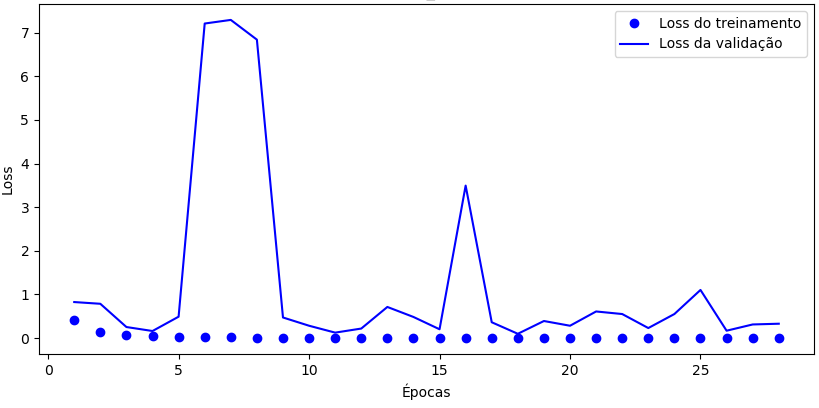
\includegraphics[width=0.45\textwidth]{imgs/alexnet-b-loss}
 }
 \subfloat[Acurácia durante treinamento da rede AlexNet B.\label{subfig:alexnet-b-acc}]{%
 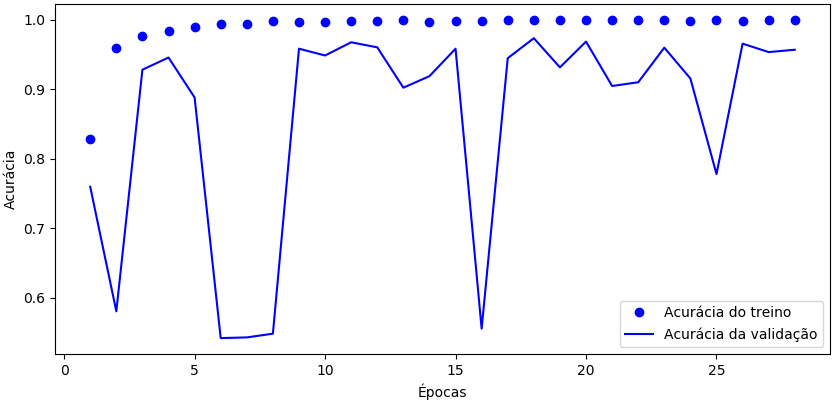
\includegraphics[width=0.45\textwidth]{imgs/alexnet-b-acc}
 }
 \hfill
 \subfloat[\emph{Loss} durante treinamento da rede AlexNet C.\label{subfig:alexnet-c-loss}]{%
 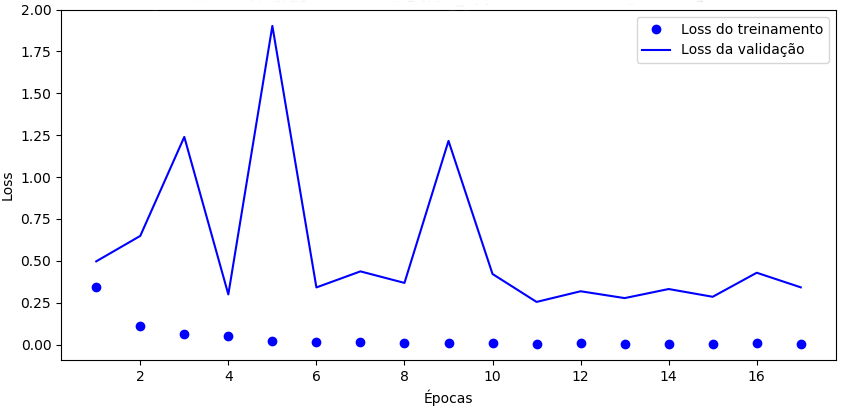
\includegraphics[width=0.45\textwidth]{imgs/alexnet-c-loss}
 }
 \subfloat[Acurácia durante treinamento da rede AlexNet C.\label{subfig:alexnet-c-acc}]{%
 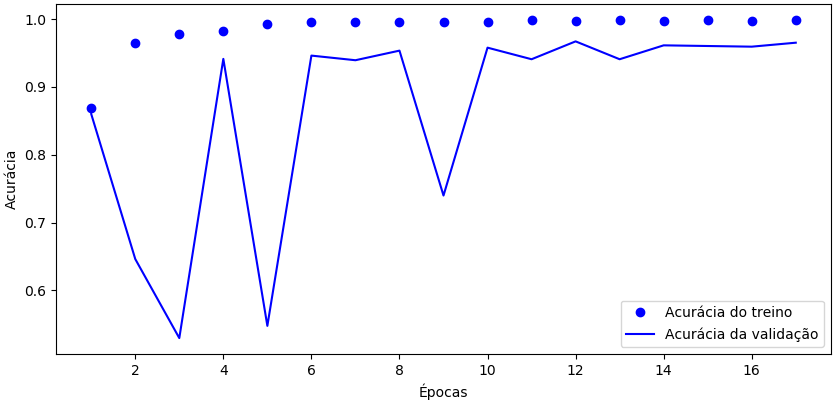
\includegraphics[width=0.45\textwidth]{imgs/alexnet-c-acc}
 }
\end{figure}

Considerando que estas redes possuem mais parâmetros treináveis, este possivelmente foi um fator responsável pelo maior números de épocas no treinamento. Nota-se ainda que houve oscilações nos treinamentos, resultando em parada precoce. Para esta arquitetura, as redes treinadas com otimizador SGD mostraram métricas melhores na etapa de avaliação.

Observando as métricas de acurácia e F-Score obtidas, percebe-se que estas foram inferiores às observadas para as redes LeNet, mas ainda assim alcançando valores superiores a $90\%$. As mesmas reflexões sobre a disposição dos valores na matriz de confusão observados no cenário LeNet se mostram cabíveis, porém com menos acertos.

\begin{figure}[H]
 \centering
 \caption{Matrizes de confusão dos melhores modelos obtidos com a arquitetura AlexNet.}
 \subfloat[AlexNet A\label{subfig:matriz-alexnet-a}]{%
 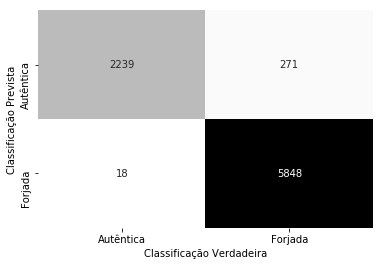
\includegraphics[width=0.5\textwidth]{imgs/matriz-alexnet-a}
 }
 \subfloat[AlexNet B\label{subfig:matriz-alexnet-b}]{%
 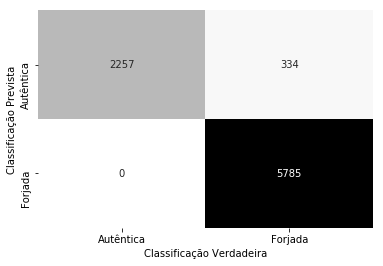
\includegraphics[width=0.5\textwidth]{imgs/matriz-alexnet-b}
 }
 \hfill
 \subfloat[AlexNet C\label{subfig:matriz-alexnet-c}]{%
 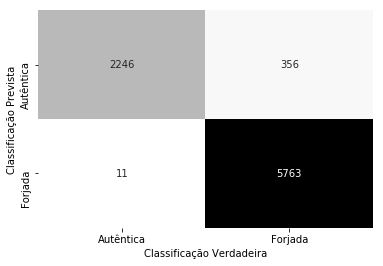
\includegraphics[width=0.5\textwidth]{imgs/matriz-alexnet-c}
 }
 \label{fig:matrizes-alexnet}
\end{figure}

De modo geral, apesar de possuir boas métricas, o melhor modelo encontrado pela arquitetura AlexNet, com um \emph{F-score} de $0.9393$, não foi suficiente para superar o melhor modelo obtido com a arquitetura LeNet ($0.9755$). Uma vez que a arquitetura LeNet possui menos parâmetros que a AlexNet e melhor desempenho observado, ressalta-se a sua maior adequação para a tarefa considerada, acrescido ao fato de demandar menos recursos de tempo de treinamento e de memória para seu armazenamento.
